% Options for packages loaded elsewhere
\PassOptionsToPackage{unicode}{hyperref}
\PassOptionsToPackage{hyphens}{url}
%
\documentclass[
]{article}
\usepackage{amsmath,amssymb}
\usepackage{lmodern}
\usepackage{iftex}
\ifPDFTeX
  \usepackage[T1]{fontenc}
  \usepackage[utf8]{inputenc}
  \usepackage{textcomp} % provide euro and other symbols
\else % if luatex or xetex
  \usepackage{unicode-math}
  \defaultfontfeatures{Scale=MatchLowercase}
  \defaultfontfeatures[\rmfamily]{Ligatures=TeX,Scale=1}
\fi
% Use upquote if available, for straight quotes in verbatim environments
\IfFileExists{upquote.sty}{\usepackage{upquote}}{}
\IfFileExists{microtype.sty}{% use microtype if available
  \usepackage[]{microtype}
  \UseMicrotypeSet[protrusion]{basicmath} % disable protrusion for tt fonts
}{}
\makeatletter
\@ifundefined{KOMAClassName}{% if non-KOMA class
  \IfFileExists{parskip.sty}{%
    \usepackage{parskip}
  }{% else
    \setlength{\parindent}{0pt}
    \setlength{\parskip}{6pt plus 2pt minus 1pt}}
}{% if KOMA class
  \KOMAoptions{parskip=half}}
\makeatother
\usepackage{xcolor}
\usepackage[margin=1in]{geometry}
\usepackage{color}
\usepackage{fancyvrb}
\newcommand{\VerbBar}{|}
\newcommand{\VERB}{\Verb[commandchars=\\\{\}]}
\DefineVerbatimEnvironment{Highlighting}{Verbatim}{commandchars=\\\{\}}
% Add ',fontsize=\small' for more characters per line
\usepackage{framed}
\definecolor{shadecolor}{RGB}{248,248,248}
\newenvironment{Shaded}{\begin{snugshade}}{\end{snugshade}}
\newcommand{\AlertTok}[1]{\textcolor[rgb]{0.94,0.16,0.16}{#1}}
\newcommand{\AnnotationTok}[1]{\textcolor[rgb]{0.56,0.35,0.01}{\textbf{\textit{#1}}}}
\newcommand{\AttributeTok}[1]{\textcolor[rgb]{0.77,0.63,0.00}{#1}}
\newcommand{\BaseNTok}[1]{\textcolor[rgb]{0.00,0.00,0.81}{#1}}
\newcommand{\BuiltInTok}[1]{#1}
\newcommand{\CharTok}[1]{\textcolor[rgb]{0.31,0.60,0.02}{#1}}
\newcommand{\CommentTok}[1]{\textcolor[rgb]{0.56,0.35,0.01}{\textit{#1}}}
\newcommand{\CommentVarTok}[1]{\textcolor[rgb]{0.56,0.35,0.01}{\textbf{\textit{#1}}}}
\newcommand{\ConstantTok}[1]{\textcolor[rgb]{0.00,0.00,0.00}{#1}}
\newcommand{\ControlFlowTok}[1]{\textcolor[rgb]{0.13,0.29,0.53}{\textbf{#1}}}
\newcommand{\DataTypeTok}[1]{\textcolor[rgb]{0.13,0.29,0.53}{#1}}
\newcommand{\DecValTok}[1]{\textcolor[rgb]{0.00,0.00,0.81}{#1}}
\newcommand{\DocumentationTok}[1]{\textcolor[rgb]{0.56,0.35,0.01}{\textbf{\textit{#1}}}}
\newcommand{\ErrorTok}[1]{\textcolor[rgb]{0.64,0.00,0.00}{\textbf{#1}}}
\newcommand{\ExtensionTok}[1]{#1}
\newcommand{\FloatTok}[1]{\textcolor[rgb]{0.00,0.00,0.81}{#1}}
\newcommand{\FunctionTok}[1]{\textcolor[rgb]{0.00,0.00,0.00}{#1}}
\newcommand{\ImportTok}[1]{#1}
\newcommand{\InformationTok}[1]{\textcolor[rgb]{0.56,0.35,0.01}{\textbf{\textit{#1}}}}
\newcommand{\KeywordTok}[1]{\textcolor[rgb]{0.13,0.29,0.53}{\textbf{#1}}}
\newcommand{\NormalTok}[1]{#1}
\newcommand{\OperatorTok}[1]{\textcolor[rgb]{0.81,0.36,0.00}{\textbf{#1}}}
\newcommand{\OtherTok}[1]{\textcolor[rgb]{0.56,0.35,0.01}{#1}}
\newcommand{\PreprocessorTok}[1]{\textcolor[rgb]{0.56,0.35,0.01}{\textit{#1}}}
\newcommand{\RegionMarkerTok}[1]{#1}
\newcommand{\SpecialCharTok}[1]{\textcolor[rgb]{0.00,0.00,0.00}{#1}}
\newcommand{\SpecialStringTok}[1]{\textcolor[rgb]{0.31,0.60,0.02}{#1}}
\newcommand{\StringTok}[1]{\textcolor[rgb]{0.31,0.60,0.02}{#1}}
\newcommand{\VariableTok}[1]{\textcolor[rgb]{0.00,0.00,0.00}{#1}}
\newcommand{\VerbatimStringTok}[1]{\textcolor[rgb]{0.31,0.60,0.02}{#1}}
\newcommand{\WarningTok}[1]{\textcolor[rgb]{0.56,0.35,0.01}{\textbf{\textit{#1}}}}
\usepackage{graphicx}
\makeatletter
\def\maxwidth{\ifdim\Gin@nat@width>\linewidth\linewidth\else\Gin@nat@width\fi}
\def\maxheight{\ifdim\Gin@nat@height>\textheight\textheight\else\Gin@nat@height\fi}
\makeatother
% Scale images if necessary, so that they will not overflow the page
% margins by default, and it is still possible to overwrite the defaults
% using explicit options in \includegraphics[width, height, ...]{}
\setkeys{Gin}{width=\maxwidth,height=\maxheight,keepaspectratio}
% Set default figure placement to htbp
\makeatletter
\def\fps@figure{htbp}
\makeatother
\setlength{\emergencystretch}{3em} % prevent overfull lines
\providecommand{\tightlist}{%
  \setlength{\itemsep}{0pt}\setlength{\parskip}{0pt}}
\setcounter{secnumdepth}{-\maxdimen} % remove section numbering
\ifLuaTeX
  \usepackage{selnolig}  % disable illegal ligatures
\fi
\IfFileExists{bookmark.sty}{\usepackage{bookmark}}{\usepackage{hyperref}}
\IfFileExists{xurl.sty}{\usepackage{xurl}}{} % add URL line breaks if available
\urlstyle{same} % disable monospaced font for URLs
\hypersetup{
  pdftitle={Parking infractions, City of Toronto take home assignment},
  pdfauthor={Nima Jamshidi},
  hidelinks,
  pdfcreator={LaTeX via pandoc}}

\title{Parking infractions, City of Toronto take home assignment}
\author{Nima Jamshidi}
\date{}

\begin{document}
\maketitle

{
\setcounter{tocdepth}{2}
\tableofcontents
}
In this notebook, I am going to study the most frequent parking
infractions in Toronto with analyzing their locations and underlying
factors. For this study, I'm using R programming language with the use
of RStudio IDE.

First step is to install and load the required packages.

\begin{Shaded}
\begin{Highlighting}[]
\CommentTok{\# suppressPackageStartupMessages(library(httr))}
\CommentTok{\# suppressPackageStartupMessages(library(jsonlite))}
\CommentTok{\#install.packages("opendatatoronto")}
\FunctionTok{suppressPackageStartupMessages}\NormalTok{(}\FunctionTok{library}\NormalTok{(opendatatoronto))}
\FunctionTok{suppressPackageStartupMessages}\NormalTok{(}\FunctionTok{library}\NormalTok{(ckanr))}
\CommentTok{\#\textgreater{} Loading required package: DBI}
\FunctionTok{suppressPackageStartupMessages}\NormalTok{(}\FunctionTok{library}\NormalTok{(readr))}
\FunctionTok{suppressPackageStartupMessages}\NormalTok{(}\FunctionTok{library}\NormalTok{(vroom))}
\FunctionTok{suppressPackageStartupMessages}\NormalTok{(}\FunctionTok{library}\NormalTok{(tidyverse))}
\FunctionTok{suppressPackageStartupMessages}\NormalTok{(}\FunctionTok{library}\NormalTok{(sf))}
\FunctionTok{suppressPackageStartupMessages}\NormalTok{(}\FunctionTok{library}\NormalTok{(leaflet))}
\FunctionTok{suppressPackageStartupMessages}\NormalTok{(}\FunctionTok{library}\NormalTok{(rjson))}
\FunctionTok{suppressPackageStartupMessages}\NormalTok{(}\FunctionTok{library}\NormalTok{(scales))}
\end{Highlighting}
\end{Shaded}

\begin{Shaded}
\begin{Highlighting}[]
\NormalTok{PaTi\_metadata }\OtherTok{\textless{}{-}}\NormalTok{ opendatatoronto}\SpecialCharTok{::}\FunctionTok{show\_package}\NormalTok{(}\StringTok{"https://open.toronto.ca/dataset/parking{-}tickets/"}\NormalTok{)}
\NormalTok{PaTi\_list }\OtherTok{\textless{}{-}}\NormalTok{ opendatatoronto}\SpecialCharTok{::}\FunctionTok{list\_package\_resources}\NormalTok{(}\StringTok{"https://open.toronto.ca/dataset/parking{-}tickets/"}\NormalTok{)}
\NormalTok{PaTi\_data\_tot }\OtherTok{\textless{}{-}} \FunctionTok{tibble}\NormalTok{()}
\NormalTok{Col\_type }\OtherTok{\textless{}{-}} \FunctionTok{cols}\NormalTok{(}
        \AttributeTok{tag\_number\_masked =} \FunctionTok{col\_character}\NormalTok{(),}
        \AttributeTok{date\_of\_infraction =} \FunctionTok{col\_double}\NormalTok{(),}
        \AttributeTok{infraction\_code =} \FunctionTok{col\_double}\NormalTok{(),}
        \AttributeTok{infraction\_description =} \FunctionTok{col\_character}\NormalTok{(),}
        \AttributeTok{set\_fine\_amount =} \FunctionTok{col\_double}\NormalTok{(),}
        \AttributeTok{time\_of\_infraction =} \FunctionTok{col\_character}\NormalTok{(),}
        \AttributeTok{location1 =} \FunctionTok{col\_character}\NormalTok{(),}
        \AttributeTok{location2 =} \FunctionTok{col\_character}\NormalTok{(),}
        \AttributeTok{location3 =} \FunctionTok{col\_character}\NormalTok{(),}
        \AttributeTok{location4 =} \FunctionTok{col\_character}\NormalTok{(),}
        \AttributeTok{province =} \FunctionTok{col\_character}\NormalTok{()}
\NormalTok{      )}

\CommentTok{\# https://github.com/tidyverse/vroom/issues/138}
\NormalTok{Corrupted\_csv }\OtherTok{\textless{}{-}} \ControlFlowTok{function}\NormalTok{(dir,PaTi\_data\_id,save\_path,Col\_type) \{}
\NormalTok{  resource\_dir }\OtherTok{\textless{}{-}}\NormalTok{ fs}\SpecialCharTok{::}\FunctionTok{dir\_create}\NormalTok{(}\FunctionTok{paste0}\NormalTok{(dir, }\StringTok{"/"}\NormalTok{, PaTi\_data\_id))}
\NormalTok{  csv\_files }\OtherTok{\textless{}{-}} \FunctionTok{unzip}\NormalTok{(save\_path[[}\StringTok{"path"}\NormalTok{]], }\AttributeTok{exdir =}\NormalTok{ resource\_dir)}
\NormalTok{  con }\OtherTok{\textless{}{-}} \FunctionTok{file}\NormalTok{(csv\_files, }\StringTok{"rb"}\NormalTok{)}
\NormalTok{  x }\OtherTok{\textless{}{-}} \FunctionTok{readBin}\NormalTok{(con, }\StringTok{"raw"}\NormalTok{, }\AttributeTok{n =} \DecValTok{500000000}\NormalTok{)}
\NormalTok{  utf\_text }\OtherTok{\textless{}{-}} \FunctionTok{iconv}\NormalTok{(}
        \FunctionTok{list}\NormalTok{(x),}
        \AttributeTok{from =} \StringTok{"UTF{-}16LE"}\NormalTok{,}
        \AttributeTok{to =} \StringTok{"UTF{-}8"}\NormalTok{,}
        \AttributeTok{toRaw =}\NormalTok{ F}
\NormalTok{      )}
\NormalTok{  res }\OtherTok{\textless{}{-}}
\NormalTok{    vroom}\SpecialCharTok{::}\FunctionTok{vroom}\NormalTok{(}
\NormalTok{      utf\_text,}
      \AttributeTok{delim =} \StringTok{","}\NormalTok{,}
      \AttributeTok{col\_types =}\NormalTok{ Col\_type,}
      \AttributeTok{col\_names =} \FunctionTok{names}\NormalTok{(Col\_type}\SpecialCharTok{$}\NormalTok{cols),}
      \AttributeTok{skip =} \DecValTok{1}
\NormalTok{    ) }\SpecialCharTok{\%\textgreater{}\%} 
    \FunctionTok{mutate}\NormalTok{(}\AttributeTok{time\_of\_infraction =} \FunctionTok{replace\_na}\NormalTok{(time\_of\_infraction, }\StringTok{"0000"}\NormalTok{))}
  \FunctionTok{return}\NormalTok{(res)}
\NormalTok{\}}

\NormalTok{read\_all\_zip }\OtherTok{\textless{}{-}} \ControlFlowTok{function}\NormalTok{(file, ...) \{}
\NormalTok{  filenames }\OtherTok{\textless{}{-}} \FunctionTok{unzip}\NormalTok{(file, }\AttributeTok{list =} \ConstantTok{TRUE}\NormalTok{)}\SpecialCharTok{$}\NormalTok{Name}
  \FunctionTok{vroom}\NormalTok{(purrr}\SpecialCharTok{::}\FunctionTok{map}\NormalTok{(filenames, }\SpecialCharTok{\textasciitilde{}} \FunctionTok{unz}\NormalTok{(file, .x)), ...)}
\NormalTok{\}}

\NormalTok{PaTi\_retrieve }\OtherTok{\textless{}{-}} \ControlFlowTok{function}\NormalTok{(i)\{}
\NormalTok{  PaTi\_data\_id }\OtherTok{\textless{}{-}}\NormalTok{ PaTi\_list[[i,}\StringTok{"id"}\NormalTok{]]}
\NormalTok{  resource }\OtherTok{\textless{}{-}}
    \FunctionTok{resource\_show}\NormalTok{(PaTi\_data\_id, }\AttributeTok{url =} \StringTok{"https://ckan0.cf.opendata.inter.prod{-}toronto.ca/"}\NormalTok{, }\AttributeTok{as =} \StringTok{"list"}\NormalTok{)}
\NormalTok{  dir }\OtherTok{\textless{}{-}} \FunctionTok{tempdir}\NormalTok{()}
\NormalTok{  resource\_dir }\OtherTok{\textless{}{-}}\NormalTok{ fs}\SpecialCharTok{::}\FunctionTok{dir\_create}\NormalTok{(}\FunctionTok{paste0}\NormalTok{(dir, }\StringTok{"/"}\NormalTok{, PaTi\_data\_id))}
\NormalTok{  save\_path }\OtherTok{\textless{}{-}}
    \FunctionTok{ckan\_fetch}\NormalTok{(}
\NormalTok{      resource[[}\StringTok{"url"}\NormalTok{]],}
      \AttributeTok{store =} \StringTok{"disk"}\NormalTok{,}
      \AttributeTok{path =} \FunctionTok{paste0}\NormalTok{(dir, }\StringTok{"/"}\NormalTok{, PaTi\_data\_id, }\StringTok{"/"}\NormalTok{, }\StringTok{"res.zip"}\NormalTok{)}
\NormalTok{    )}
\NormalTok{  t }\OtherTok{\textless{}{-}} \FunctionTok{try}\NormalTok{(\{}
    \CommentTok{\# https://github.com/tidyverse/vroom/issues/125}
\NormalTok{    filenames }\OtherTok{\textless{}{-}} \FunctionTok{unzip}\NormalTok{(save\_path}\SpecialCharTok{$}\NormalTok{path, }\AttributeTok{list =} \ConstantTok{TRUE}\NormalTok{)}\SpecialCharTok{$}\NormalTok{Name}
\NormalTok{    res }\OtherTok{\textless{}{-}} \FunctionTok{bind\_rows}\NormalTok{(purrr}\SpecialCharTok{::}\FunctionTok{map}\NormalTok{(filenames, }\SpecialCharTok{\textasciitilde{}} \FunctionTok{vroom}\NormalTok{(}\FunctionTok{unz}\NormalTok{(save\_path}\SpecialCharTok{$}\NormalTok{path, .x),}
                                                   \AttributeTok{delim =} \StringTok{","}\NormalTok{,}
                                                   \AttributeTok{col\_names =} \FunctionTok{names}\NormalTok{(Col\_type}\SpecialCharTok{$}\NormalTok{cols),}
                                                   \AttributeTok{col\_types =}\NormalTok{ Col\_type,}
                                                   \AttributeTok{skip =} \DecValTok{1}\NormalTok{)))}
\NormalTok{  \})}
  \ControlFlowTok{if}\NormalTok{ (}\FunctionTok{inherits}\NormalTok{(t, }\StringTok{"try{-}error"}\NormalTok{)}\SpecialCharTok{|}\FunctionTok{ncol}\NormalTok{(res)}\SpecialCharTok{!=}\DecValTok{11}\NormalTok{)  \{}
    \FunctionTok{print}\NormalTok{(}\StringTok{"corrupted CSV"}\NormalTok{)}
\NormalTok{    res }\OtherTok{\textless{}{-}} \FunctionTok{Corrupted\_csv}\NormalTok{(dir,PaTi\_data\_id,save\_path,Col\_type)\}}
  \FunctionTok{unlink}\NormalTok{(dir)}
  \FunctionTok{return}\NormalTok{(res)}
\NormalTok{\}}
\end{Highlighting}
\end{Shaded}

\begin{Shaded}
\begin{Highlighting}[]
\ControlFlowTok{for}\NormalTok{ (i }\ControlFlowTok{in} \FunctionTok{str\_which}\NormalTok{(PaTi\_list}\SpecialCharTok{$}\NormalTok{name, }\StringTok{"parking{-}tickets{-}}\SpecialCharTok{\textbackslash{}\textbackslash{}}\StringTok{d"}\NormalTok{)) \{}
  \FunctionTok{print}\NormalTok{(}\FunctionTok{paste}\NormalTok{(}\FunctionTok{str\_extract}\NormalTok{(PaTi\_list}\SpecialCharTok{$}\NormalTok{name[i],}\StringTok{"}\SpecialCharTok{\textbackslash{}\textbackslash{}}\StringTok{d+"}\NormalTok{),}\StringTok{"started."}\NormalTok{))}
\NormalTok{  res }\OtherTok{\textless{}{-}} \FunctionTok{PaTi\_retrieve}\NormalTok{(i)}
  \FunctionTok{print}\NormalTok{(}\FunctionTok{paste}\NormalTok{(}\FunctionTok{str\_extract}\NormalTok{(PaTi\_list}\SpecialCharTok{$}\NormalTok{name[i],}\StringTok{"}\SpecialCharTok{\textbackslash{}\textbackslash{}}\StringTok{d+"}\NormalTok{),}\StringTok{"retrieval done!"}\NormalTok{))}
\NormalTok{  PaTi\_data\_tot }\OtherTok{\textless{}{-}}\NormalTok{ PaTi\_data\_tot }\SpecialCharTok{\%\textgreater{}\%} \FunctionTok{rbind}\NormalTok{(res)}
\NormalTok{\}}
\FunctionTok{rm}\NormalTok{(Col\_type,Pati\_list,res,i,Corrupted\_csv)}
\FunctionTok{saveRDS}\NormalTok{(PaTi\_data\_tot,}\StringTok{"PaTi\_data\_tot.rds"}\NormalTok{)}
\end{Highlighting}
\end{Shaded}

\begin{Shaded}
\begin{Highlighting}[]
\NormalTok{PaTi\_data\_tot }\OtherTok{\textless{}{-}} \FunctionTok{readRDS}\NormalTok{(}\StringTok{"PaTi\_data\_tot.rds"}\NormalTok{) }\SpecialCharTok{\%\textgreater{}\%} \FunctionTok{filter}\NormalTok{(date\_of\_infraction}\SpecialCharTok{\textgreater{}}\DecValTok{20200000}\NormalTok{)}
\end{Highlighting}
\end{Shaded}

\begin{Shaded}
\begin{Highlighting}[]
\NormalTok{Pati\_rank }\OtherTok{\textless{}{-}}\NormalTok{ PaTi\_data\_tot }\SpecialCharTok{\%\textgreater{}\%} 
  \FunctionTok{group\_by}\NormalTok{(infraction\_code, infraction\_description) }\SpecialCharTok{\%\textgreater{}\%} 
  \FunctionTok{summarise}\NormalTok{(}\AttributeTok{n =} \FunctionTok{n}\NormalTok{()) }\SpecialCharTok{\%\textgreater{}\%} 
  \FunctionTok{mutate}\NormalTok{(}\AttributeTok{n\_tot =} \FunctionTok{sum}\NormalTok{(n),}
         \AttributeTok{infraction\_description2 =}\NormalTok{ infraction\_description[}\FunctionTok{which.max}\NormalTok{(}\FunctionTok{nchar}\NormalTok{(infraction\_description))],}
         \AttributeTok{row\_num =} \FunctionTok{row\_number}\NormalTok{()) }\SpecialCharTok{\%\textgreater{}\%} 
  \FunctionTok{filter}\NormalTok{(row\_num }\SpecialCharTok{==} \DecValTok{1}\NormalTok{) }\SpecialCharTok{\%\textgreater{}\%} 
  \FunctionTok{select}\NormalTok{(}\SpecialCharTok{{-}}\NormalTok{n, }\SpecialCharTok{{-}}\NormalTok{infraction\_description2,}\SpecialCharTok{{-}}\NormalTok{row\_num) }\SpecialCharTok{\%\textgreater{}\%} 
  \FunctionTok{arrange}\NormalTok{(}\FunctionTok{desc}\NormalTok{(n\_tot))}
\end{Highlighting}
\end{Shaded}

\begin{verbatim}
## `summarise()` has grouped output by 'infraction_code'. You can override using
## the `.groups` argument.
\end{verbatim}

\begin{Shaded}
\begin{Highlighting}[]
\NormalTok{GeoC\_metadata }\OtherTok{\textless{}{-}}\NormalTok{ opendatatoronto}\SpecialCharTok{::}\FunctionTok{show\_package}\NormalTok{(}\StringTok{"https://open.toronto.ca/dataset/address{-}points{-}municipal{-}toronto{-}one{-}address{-}repository/"}\NormalTok{)}
\NormalTok{GeoC\_list }\OtherTok{\textless{}{-}}\NormalTok{ opendatatoronto}\SpecialCharTok{::}\FunctionTok{list\_package\_resources}\NormalTok{(}\StringTok{"https://open.toronto.ca/dataset/address{-}points{-}municipal{-}toronto{-}one{-}address{-}repository/"}\NormalTok{)}
\NormalTok{GeoC\_retrieve }\OtherTok{\textless{}{-}} \ControlFlowTok{function}\NormalTok{() \{}
\NormalTok{  GeoC\_data\_id }\OtherTok{\textless{}{-}}\NormalTok{ GeoC\_list[[}\DecValTok{3}\NormalTok{, }\StringTok{"id"}\NormalTok{]]}
\NormalTok{  resource }\OtherTok{\textless{}{-}}
    \FunctionTok{resource\_show}\NormalTok{(GeoC\_data\_id, }\AttributeTok{url =} \StringTok{"https://ckan0.cf.opendata.inter.prod{-}toronto.ca/"}\NormalTok{, }\AttributeTok{as =} \StringTok{"list"}\NormalTok{)}
\NormalTok{  dir }\OtherTok{\textless{}{-}} \FunctionTok{tempdir}\NormalTok{()}
\NormalTok{  resource\_dir }\OtherTok{\textless{}{-}}\NormalTok{ fs}\SpecialCharTok{::}\FunctionTok{dir\_create}\NormalTok{(}\FunctionTok{paste0}\NormalTok{(dir, }\StringTok{"/"}\NormalTok{, GeoC\_data\_id))}
\NormalTok{  save\_path }\OtherTok{\textless{}{-}}
    \FunctionTok{ckan\_fetch}\NormalTok{(}
\NormalTok{      resource[[}\StringTok{"url"}\NormalTok{]],}
      \AttributeTok{store =} \StringTok{"disk"}\NormalTok{,}
      \AttributeTok{path =} \FunctionTok{paste0}\NormalTok{(dir, }\StringTok{"/"}\NormalTok{, GeoC\_data\_id, }\StringTok{"/"}\NormalTok{, }\StringTok{"res.zip"}\NormalTok{)}
\NormalTok{    )}
\NormalTok{  GeoC\_files }\OtherTok{\textless{}{-}} \FunctionTok{unzip}\NormalTok{(save\_path[[}\StringTok{"path"}\NormalTok{]], }\AttributeTok{exdir =}\NormalTok{ resource\_dir)}
\NormalTok{  GeoC\_shp }\OtherTok{\textless{}{-}} \FunctionTok{st\_read}\NormalTok{(GeoC\_files[}\FunctionTok{str\_ends}\NormalTok{(GeoC\_files, }\StringTok{".shp"}\NormalTok{)])}
\NormalTok{\}}

\NormalTok{GeoC\_shp }\OtherTok{\textless{}{-}} \FunctionTok{GeoC\_retrieve}\NormalTok{()}
\end{Highlighting}
\end{Shaded}

\begin{verbatim}
## Reading layer `ADDRESS_POINT_WGS84' from data source 
##   `C:\Users\nimad\AppData\Local\Temp\Rtmp2BtY4T\eba07dba-8645-45f8-950c-0381a0dcaa1b\ADDRESS_POINT_WGS84.shp' 
##   using driver `ESRI Shapefile'
## Simple feature collection with 525368 features and 22 fields
## Geometry type: POINT
## Dimension:     XY
## Bounding box:  xmin: -8865288 ymin: 5401672 xmax: -8807754 ymax: 5442900
## Projected CRS: WGS 84 / Pseudo-Mercator
\end{verbatim}

\begin{Shaded}
\begin{Highlighting}[]
\NormalTok{GeoC\_shp }\OtherTok{\textless{}{-}}\NormalTok{ GeoC\_shp }\SpecialCharTok{\%\textgreater{}\%} \FunctionTok{mutate}\NormalTok{(}\AttributeTok{LFNAME\_lower =} \FunctionTok{tolower}\NormalTok{(LFNAME))}
\end{Highlighting}
\end{Shaded}

\begin{Shaded}
\begin{Highlighting}[]
\NormalTok{PaTi\_data\_top20\_split }\OtherTok{\textless{}{-}}\NormalTok{ PaTi\_data\_tot }\SpecialCharTok{\%\textgreater{}\%}
  \FunctionTok{filter}\NormalTok{(infraction\_code }\SpecialCharTok{\%in\%}\NormalTok{ Pati\_rank}\SpecialCharTok{$}\NormalTok{infraction\_code[}\DecValTok{1}\SpecialCharTok{:}\DecValTok{20}\NormalTok{]) }\SpecialCharTok{\%\textgreater{}\%} 
  \FunctionTok{mutate}\NormalTok{(}\AttributeTok{group =} \FunctionTok{grepl}\NormalTok{(}\StringTok{\textquotesingle{}\^{}[[:punct:]]?}\SpecialCharTok{\textbackslash{}\textbackslash{}}\StringTok{d\textquotesingle{}}\NormalTok{, location2))}

\NormalTok{PaTi\_data\_top20\_1 }\OtherTok{\textless{}{-}}\NormalTok{  PaTi\_data\_top20\_split[PaTi\_data\_top20\_split}\SpecialCharTok{$}\NormalTok{group,] }\SpecialCharTok{\%\textgreater{}\%} 
  \FunctionTok{group\_by}\NormalTok{(infraction\_code,location2) }\SpecialCharTok{\%\textgreater{}\%} 
  \FunctionTok{summarise}\NormalTok{(}\AttributeTok{n=}\FunctionTok{n}\NormalTok{()) }\SpecialCharTok{\%\textgreater{}\%} 
  \FunctionTok{rowwise}\NormalTok{() }\SpecialCharTok{\%\textgreater{}\%}
  \FunctionTok{mutate}\NormalTok{(}\AttributeTok{ADDRESS =} \FunctionTok{str\_extract}\NormalTok{(}\FunctionTok{str\_extract}\NormalTok{(location2,}\StringTok{"\^{}[:punct:]?}\SpecialCharTok{\textbackslash{}\textbackslash{}}\StringTok{d*((?\textless{}=}\SpecialCharTok{\textbackslash{}\textbackslash{}}\StringTok{d)[:alpha:](?=}\SpecialCharTok{\textbackslash{}\textbackslash{}}\StringTok{s))?"}\NormalTok{),}\StringTok{"[\^{}[:punct:]]+"}\NormalTok{),}
         \AttributeTok{LFNAME\_lower =} \FunctionTok{tolower}\NormalTok{(}\FunctionTok{str\_trim}\NormalTok{(}\FunctionTok{sub}\NormalTok{(ADDRESS,}\StringTok{""}\NormalTok{,location2)))) }\SpecialCharTok{\%\textgreater{}\%} 
  \FunctionTok{left\_join}\NormalTok{((GeoC\_shp }\SpecialCharTok{\%\textgreater{}\%} \FunctionTok{select}\NormalTok{(GEO\_ID,LINK,LFNAME\_lower,ADDRESS)),}\AttributeTok{by =} \FunctionTok{c}\NormalTok{(}\StringTok{"LFNAME\_lower"}\NormalTok{,}\StringTok{"ADDRESS"}\NormalTok{)) }\SpecialCharTok{\%\textgreater{}\%} 
  \FunctionTok{group\_by}\NormalTok{(infraction\_code, LINK) }\SpecialCharTok{\%\textgreater{}\%}
  \FunctionTok{summarise}\NormalTok{(}\AttributeTok{n =} \FunctionTok{sum}\NormalTok{(n,}\AttributeTok{na.rm =} \ConstantTok{TRUE}\NormalTok{)) }\SpecialCharTok{\%\textgreater{}\%} 
  \FunctionTok{mutate}\NormalTok{(}\AttributeTok{accurate\_type =}\NormalTok{ T,}
         \AttributeTok{reference\_type =} \StringTok{"LINK"}\NormalTok{) }\SpecialCharTok{\%\textgreater{}\%} 
  \FunctionTok{rename}\NormalTok{(}\AttributeTok{reference =}\NormalTok{ LINK)}
\end{Highlighting}
\end{Shaded}

\begin{verbatim}
## `summarise()` has grouped output by 'infraction_code'. You can override using
## the `.groups` argument.
## `summarise()` has grouped output by 'infraction_code'. You can override using
## the `.groups` argument.
\end{verbatim}

\begin{Shaded}
\begin{Highlighting}[]
\NormalTok{PaTi\_data\_top20\_2 }\OtherTok{\textless{}{-}}\NormalTok{ PaTi\_data\_top20\_split[}\SpecialCharTok{!}\NormalTok{PaTi\_data\_top20\_split}\SpecialCharTok{$}\NormalTok{group,] }\SpecialCharTok{\%\textgreater{}\%}  
  \FunctionTok{group\_by}\NormalTok{(infraction\_code,location2,location4) }\SpecialCharTok{\%\textgreater{}\%} 
  \FunctionTok{summarise}\NormalTok{(}\AttributeTok{n=}\FunctionTok{n}\NormalTok{()) }\SpecialCharTok{\%\textgreater{}\%} 
  \FunctionTok{rowwise}\NormalTok{() }\SpecialCharTok{\%\textgreater{}\%}
  \FunctionTok{mutate}\NormalTok{(}\AttributeTok{location2 =} \FunctionTok{tolower}\NormalTok{(}\FunctionTok{str\_trim}\NormalTok{(location2)),}
         \AttributeTok{location4 =} \FunctionTok{tolower}\NormalTok{(}\FunctionTok{str\_trim}\NormalTok{(location4)))}
\end{Highlighting}
\end{Shaded}

\begin{verbatim}
## `summarise()` has grouped output by 'infraction_code', 'location2'. You can
## override using the `.groups` argument.
\end{verbatim}

\begin{Shaded}
\begin{Highlighting}[]
\NormalTok{Intersection\_geocoder }\OtherTok{\textless{}{-}} \ControlFlowTok{function}\NormalTok{(location2,location4)\{}
\NormalTok{  shp1 }\OtherTok{\textless{}{-}}\NormalTok{ GeoC\_shp }\SpecialCharTok{\%\textgreater{}\%} 
    \FunctionTok{filter}\NormalTok{(LFNAME\_lower }\SpecialCharTok{==}\NormalTok{ location2)}
  \ControlFlowTok{if}\NormalTok{ (}\FunctionTok{nrow}\NormalTok{(shp1)}\SpecialCharTok{==}\DecValTok{0}\NormalTok{)\{}\FunctionTok{return}\NormalTok{(}\ConstantTok{NA}\NormalTok{)\}}
\NormalTok{  shp1 }\OtherTok{\textless{}{-}}\NormalTok{ shp1 }\SpecialCharTok{\%\textgreater{}\%} \FunctionTok{group\_by}\NormalTok{(LINK) }\SpecialCharTok{\%\textgreater{}\%} 
    \FunctionTok{filter}\NormalTok{(DISTANCE }\SpecialCharTok{\%in\%} \FunctionTok{c}\NormalTok{(}\FunctionTok{min}\NormalTok{(DISTANCE),}\FunctionTok{max}\NormalTok{(DISTANCE)))}
  
\NormalTok{  shp2 }\OtherTok{\textless{}{-}}\NormalTok{ GeoC\_shp }\SpecialCharTok{\%\textgreater{}\%} 
    \FunctionTok{filter}\NormalTok{(LFNAME\_lower }\SpecialCharTok{==}\NormalTok{ location4) }
  \ControlFlowTok{if}\NormalTok{ (}\FunctionTok{nrow}\NormalTok{(shp2)}\SpecialCharTok{==}\DecValTok{0}\NormalTok{)\{}\FunctionTok{return}\NormalTok{(}\ConstantTok{NA}\NormalTok{)\}}
\NormalTok{  shp2 }\OtherTok{\textless{}{-}}\NormalTok{ shp2 }\SpecialCharTok{\%\textgreater{}\%} \FunctionTok{group\_by}\NormalTok{(LINK) }\SpecialCharTok{\%\textgreater{}\%} 
    \FunctionTok{filter}\NormalTok{(DISTANCE }\SpecialCharTok{\%in\%} \FunctionTok{c}\NormalTok{(}\FunctionTok{min}\NormalTok{(DISTANCE),}\FunctionTok{max}\NormalTok{(DISTANCE)))}
  
\NormalTok{  dist }\OtherTok{=} \FunctionTok{st\_distance}\NormalTok{(shp1,shp2)}
\NormalTok{  ind }\OtherTok{=} \FunctionTok{which}\NormalTok{(dist }\SpecialCharTok{==} \FunctionTok{min}\NormalTok{(dist), }\AttributeTok{arr.ind =} \ConstantTok{TRUE}\NormalTok{)}
\NormalTok{  location }\OtherTok{=}\NormalTok{ shp1[ind[}\DecValTok{1}\NormalTok{],][[}\StringTok{"GEO\_ID"}\NormalTok{]]}
  \FunctionTok{return}\NormalTok{(location)}
\NormalTok{\}}

\NormalTok{GeoC\_shp\_intersection }\OtherTok{\textless{}{-}}\NormalTok{ PaTi\_data\_top20\_2 }\SpecialCharTok{\%\textgreater{}\%} \FunctionTok{ungroup}\NormalTok{() }\SpecialCharTok{\%\textgreater{}\%} \FunctionTok{select}\NormalTok{(location2,location4) }\SpecialCharTok{\%\textgreater{}\%} \FunctionTok{distinct}\NormalTok{() }\SpecialCharTok{\%\textgreater{}\%} 
  \FunctionTok{mutate}\NormalTok{(}\AttributeTok{GEO\_ID =}\NormalTok{ purrr}\SpecialCharTok{::}\FunctionTok{map2\_dbl}\NormalTok{(location2,location2,Intersection\_geocoder))}

\FunctionTok{saveRDS}\NormalTok{(GeoC\_shp\_intersection,}\StringTok{"GeoC\_shp\_intersection.rds"}\NormalTok{)}
\end{Highlighting}
\end{Shaded}

\begin{Shaded}
\begin{Highlighting}[]
\NormalTok{GeoC\_shp\_intersection }\OtherTok{\textless{}{-}} \FunctionTok{readRDS}\NormalTok{(}\StringTok{"GeoC\_shp\_intersection.rds"}\NormalTok{)}


\NormalTok{PaTi\_data\_top20\_2 }\OtherTok{\textless{}{-}}\NormalTok{ PaTi\_data\_top20\_2 }\SpecialCharTok{\%\textgreater{}\%} \FunctionTok{left\_join}\NormalTok{(GeoC\_shp\_intersection,}\AttributeTok{by =} \FunctionTok{c}\NormalTok{(}\StringTok{"location2"}\NormalTok{,}\StringTok{"location4"}\NormalTok{)) }\SpecialCharTok{\%\textgreater{}\%} 
  \FunctionTok{group\_by}\NormalTok{(infraction\_code, GEO\_ID) }\SpecialCharTok{\%\textgreater{}\%}
  \FunctionTok{summarise}\NormalTok{(}\AttributeTok{n =} \FunctionTok{sum}\NormalTok{(n,}\AttributeTok{na.rm =} \ConstantTok{TRUE}\NormalTok{)) }\SpecialCharTok{\%\textgreater{}\%} 
  \FunctionTok{mutate}\NormalTok{(}\AttributeTok{accurate\_type =}\NormalTok{ F,}
         \AttributeTok{reference\_type =} \StringTok{"GEO\_ID"}\NormalTok{) }\SpecialCharTok{\%\textgreater{}\%} 
  \FunctionTok{rename}\NormalTok{(}\AttributeTok{reference =}\NormalTok{ GEO\_ID)}
\end{Highlighting}
\end{Shaded}

\begin{verbatim}
## `summarise()` has grouped output by 'infraction_code'. You can override using
## the `.groups` argument.
\end{verbatim}

\begin{Shaded}
\begin{Highlighting}[]
\NormalTok{PaTi\_data\_top20 }\OtherTok{\textless{}{-}}\NormalTok{ PaTi\_data\_top20\_1 }\SpecialCharTok{\%\textgreater{}\%}
  \FunctionTok{rbind}\NormalTok{(PaTi\_data\_top20\_2) }\SpecialCharTok{\%\textgreater{}\%} 
  \FunctionTok{filter}\NormalTok{(}\SpecialCharTok{!}\FunctionTok{is.na}\NormalTok{(reference)) }\SpecialCharTok{\%\textgreater{}\%} 
  \FunctionTok{group\_by}\NormalTok{(infraction\_code) }\SpecialCharTok{\%\textgreater{}\%}
  \FunctionTok{filter}\NormalTok{(n }\SpecialCharTok{==} \FunctionTok{max}\NormalTok{(n)) }\SpecialCharTok{\%\textgreater{}\%} 
  \FunctionTok{arrange}\NormalTok{(}\FunctionTok{desc}\NormalTok{(n))}
\end{Highlighting}
\end{Shaded}

\begin{Shaded}
\begin{Highlighting}[]
\NormalTok{fine\_data }\OtherTok{\textless{}{-}}\NormalTok{ PaTi\_data\_tot }\SpecialCharTok{\%\textgreater{}\%} \FunctionTok{group\_by}\NormalTok{(infraction\_code,set\_fine\_amount) }\SpecialCharTok{\%\textgreater{}\%} \FunctionTok{summarise}\NormalTok{(}\AttributeTok{n=}\FunctionTok{n}\NormalTok{()) }\SpecialCharTok{\%\textgreater{}\%} \FunctionTok{filter}\NormalTok{(n }\SpecialCharTok{==} \FunctionTok{max}\NormalTok{(n)) }\SpecialCharTok{\%\textgreater{}\%} \FunctionTok{select}\NormalTok{(}\SpecialCharTok{{-}}\NormalTok{n)}
\end{Highlighting}
\end{Shaded}

\begin{verbatim}
## `summarise()` has grouped output by 'infraction_code'. You can override using
## the `.groups` argument.
\end{verbatim}

\begin{Shaded}
\begin{Highlighting}[]
\NormalTok{PaTi\_polygon\_1 }\OtherTok{\textless{}{-}}\NormalTok{ GeoC\_shp }\SpecialCharTok{\%\textgreater{}\%} 
  \FunctionTok{inner\_join}\NormalTok{((PaTi\_data\_top20 }\SpecialCharTok{\%\textgreater{}\%}
               \FunctionTok{filter}\NormalTok{(reference\_type }\SpecialCharTok{==} \StringTok{"LINK"}\NormalTok{) }\SpecialCharTok{\%\textgreater{}\%}
               \FunctionTok{select}\NormalTok{(infraction\_code,reference,}\AttributeTok{no\_infraction =}\NormalTok{ n)),}
             \AttributeTok{by =} \FunctionTok{c}\NormalTok{(}\StringTok{"LINK"}\OtherTok{=}\StringTok{"reference"}\NormalTok{)) }\SpecialCharTok{\%\textgreater{}\%} 
  \FunctionTok{left\_join}\NormalTok{((Pati\_rank }\SpecialCharTok{\%\textgreater{}\%} \FunctionTok{select}\NormalTok{(}\FunctionTok{starts\_with}\NormalTok{(}\StringTok{"infraction"}\NormalTok{))),}\AttributeTok{by =} \StringTok{"infraction\_code"}\NormalTok{) }\SpecialCharTok{\%\textgreater{}\%} 
  \FunctionTok{group\_by}\NormalTok{(infraction\_code, no\_infraction, infraction\_description, LFNAME) }\SpecialCharTok{\%\textgreater{}\%} 
  \FunctionTok{summarise}\NormalTok{(}\AttributeTok{n\_link=}\FunctionTok{n}\NormalTok{())}
\end{Highlighting}
\end{Shaded}

\begin{verbatim}
## `summarise()` has grouped output by 'infraction_code', 'no_infraction',
## 'infraction_description'. You can override using the `.groups` argument.
\end{verbatim}

\begin{Shaded}
\begin{Highlighting}[]
\NormalTok{PaTi\_polygon\_2 }\OtherTok{\textless{}{-}}\NormalTok{ GeoC\_shp }\SpecialCharTok{\%\textgreater{}\%} 
  \FunctionTok{inner\_join}\NormalTok{((PaTi\_data\_top20 }\SpecialCharTok{\%\textgreater{}\%}
               \FunctionTok{filter}\NormalTok{(reference\_type }\SpecialCharTok{==} \StringTok{"GEO\_ID"}\NormalTok{) }\SpecialCharTok{\%\textgreater{}\%}
               \FunctionTok{select}\NormalTok{(infraction\_code,reference,}\AttributeTok{no\_infraction =}\NormalTok{ n)),}
             \AttributeTok{by =} \FunctionTok{c}\NormalTok{(}\StringTok{"GEO\_ID"}\OtherTok{=}\StringTok{"reference"}\NormalTok{)) }\SpecialCharTok{\%\textgreater{}\%} 
  \FunctionTok{left\_join}\NormalTok{((Pati\_rank }\SpecialCharTok{\%\textgreater{}\%} \FunctionTok{select}\NormalTok{(}\FunctionTok{starts\_with}\NormalTok{(}\StringTok{"infraction"}\NormalTok{))),}\AttributeTok{by =} \StringTok{"infraction\_code"}\NormalTok{) }\SpecialCharTok{\%\textgreater{}\%} 
  \FunctionTok{group\_by}\NormalTok{(infraction\_code, no\_infraction, infraction\_description, LFNAME) }\SpecialCharTok{\%\textgreater{}\%} 
  \FunctionTok{summarise}\NormalTok{(}\AttributeTok{n\_link=}\FunctionTok{n}\NormalTok{())}
\end{Highlighting}
\end{Shaded}

\begin{verbatim}
## `summarise()` has grouped output by 'infraction_code', 'no_infraction',
## 'infraction_description'. You can override using the `.groups` argument.
\end{verbatim}

\begin{Shaded}
\begin{Highlighting}[]
\NormalTok{PaTi\_polygon\_make }\OtherTok{\textless{}{-}} \ControlFlowTok{function}\NormalTok{(data) \{}
  \ControlFlowTok{if}\NormalTok{ (data}\SpecialCharTok{$}\NormalTok{n\_link[}\DecValTok{1}\NormalTok{] }\SpecialCharTok{==} \DecValTok{1}\NormalTok{) \{}
\NormalTok{    data }\SpecialCharTok{\%\textgreater{}\%}
      \CommentTok{\# summarise(n\_link = n()) \%\textgreater{}\%}
      \CommentTok{\# filter(n\_link == 1) \%\textgreater{}\%}
      \FunctionTok{st\_transform}\NormalTok{(}\DecValTok{3347}\NormalTok{) }\SpecialCharTok{\%\textgreater{}\%}
      \FunctionTok{st\_buffer}\NormalTok{(}\AttributeTok{dist =} \DecValTok{10}\NormalTok{) }\SpecialCharTok{\%\textgreater{}\%}
      \FunctionTok{st\_transform}\NormalTok{(}\DecValTok{4326}\NormalTok{) }\SpecialCharTok{\%\textgreater{}\%} 
      \FunctionTok{st\_cast}\NormalTok{(}\StringTok{"POLYGON"}\NormalTok{)}
\NormalTok{  \} }\ControlFlowTok{else} \ControlFlowTok{if}\NormalTok{ (data}\SpecialCharTok{$}\NormalTok{n\_link[}\DecValTok{1}\NormalTok{] }\SpecialCharTok{==} \DecValTok{2}\NormalTok{) \{}
\NormalTok{    data }\SpecialCharTok{\%\textgreater{}\%}
      \CommentTok{\# summarise(n\_link = n()) \%\textgreater{}\%}
      \FunctionTok{st\_cast}\NormalTok{(}\StringTok{"LINESTRING"}\NormalTok{) }\SpecialCharTok{\%\textgreater{}\%}
      \FunctionTok{st\_transform}\NormalTok{(}\DecValTok{3347}\NormalTok{) }\SpecialCharTok{\%\textgreater{}\%}
      \FunctionTok{st\_buffer}\NormalTok{(}\AttributeTok{dist =} \DecValTok{10}\NormalTok{) }\SpecialCharTok{\%\textgreater{}\%}
      \FunctionTok{st\_transform}\NormalTok{(}\DecValTok{4326}\NormalTok{)}
\NormalTok{  \} }\ControlFlowTok{else} \ControlFlowTok{if}\NormalTok{ (data}\SpecialCharTok{$}\NormalTok{n\_link[}\DecValTok{1}\NormalTok{] }\SpecialCharTok{==} \DecValTok{3}\NormalTok{) \{}
\NormalTok{    temp }\OtherTok{=}\NormalTok{ data }\SpecialCharTok{\%\textgreater{}\%} \FunctionTok{st\_coordinates}\NormalTok{()}
    \FunctionTok{st\_geometry}\NormalTok{(data) }\OtherTok{=} \FunctionTok{st\_geometry}\NormalTok{(}\FunctionTok{st\_as\_sf}\NormalTok{(}\FunctionTok{as.data.frame}\NormalTok{(temp[}\FunctionTok{c}\NormalTok{(}\DecValTok{1}\NormalTok{,}\DecValTok{1}\NormalTok{,}\DecValTok{2}\NormalTok{,}\DecValTok{3}\NormalTok{),]),}\AttributeTok{coords =} \FunctionTok{c}\NormalTok{(}\StringTok{"X"}\NormalTok{,}\StringTok{"Y"}\NormalTok{),}\AttributeTok{crs =} \FunctionTok{st\_crs}\NormalTok{(data)) }\SpecialCharTok{\%\textgreater{}\%} \FunctionTok{summarise}\NormalTok{())}
\NormalTok{    data }\SpecialCharTok{\%\textgreater{}\%} 
      \FunctionTok{st\_cast}\NormalTok{(}\StringTok{"POLYGON"}\NormalTok{) }\SpecialCharTok{\%\textgreater{}\%}
      \FunctionTok{st\_convex\_hull}\NormalTok{() }\SpecialCharTok{\%\textgreater{}\%} 
      \FunctionTok{st\_transform}\NormalTok{(}\DecValTok{4326}\NormalTok{)}
\NormalTok{  \} }\ControlFlowTok{else}\NormalTok{ \{}
\NormalTok{    data }\SpecialCharTok{\%\textgreater{}\%}
      \FunctionTok{st\_cast}\NormalTok{(}\StringTok{"POLYGON"}\NormalTok{) }\SpecialCharTok{\%\textgreater{}\%}
      \FunctionTok{st\_convex\_hull}\NormalTok{() }\SpecialCharTok{\%\textgreater{}\%} 
      \FunctionTok{st\_transform}\NormalTok{(}\DecValTok{4326}\NormalTok{)}
\NormalTok{  \}}
\NormalTok{\}}

\DocumentationTok{\#\# For some reason sf package does not let me have poygons made from point buffers be in the same df that contains regular polygons, so we split them: }

\NormalTok{PaTi\_polygon\_pl }\OtherTok{\textless{}{-}}\NormalTok{ PaTi\_polygon\_1 }\SpecialCharTok{\%\textgreater{}\%}
  \FunctionTok{rbind}\NormalTok{(PaTi\_polygon\_2) }\SpecialCharTok{\%\textgreater{}\%}
  \FunctionTok{filter}\NormalTok{(n\_link }\SpecialCharTok{\textgreater{}} \DecValTok{1}\NormalTok{) }\SpecialCharTok{\%\textgreater{}\%} 
  \FunctionTok{PaTi\_polygon\_make}\NormalTok{() }\SpecialCharTok{\%\textgreater{}\%} 
  \FunctionTok{left\_join}\NormalTok{(fine\_data,}\AttributeTok{by =} \StringTok{"infraction\_code"}\NormalTok{)}

\NormalTok{PaTi\_polygon\_pt }\OtherTok{\textless{}{-}}\NormalTok{ PaTi\_polygon\_1 }\SpecialCharTok{\%\textgreater{}\%}
  \FunctionTok{rbind}\NormalTok{(PaTi\_polygon\_2) }\SpecialCharTok{\%\textgreater{}\%}
  \FunctionTok{filter}\NormalTok{(n\_link }\SpecialCharTok{==} \DecValTok{1}\NormalTok{) }\SpecialCharTok{\%\textgreater{}\%} 
  \FunctionTok{PaTi\_polygon\_make}\NormalTok{() }\SpecialCharTok{\%\textgreater{}\%} 
  \FunctionTok{left\_join}\NormalTok{(fine\_data,}\AttributeTok{by =} \StringTok{"infraction\_code"}\NormalTok{)}
  

\CommentTok{\# leaf\_sf(tt[1,] \%\textgreater{}\% st\_transform(4326)) \%\textgreater{}\% }
\CommentTok{\#   addPolygons(data = tt2[1,],}
\CommentTok{\#               popup=paste("Stratum:",tt[1,]$infraction\_code,"\textless{}br\textgreater{}"),}
\CommentTok{\#               label = \textasciitilde{} paste0("Total Income: ", infraction\_code))}
\CommentTok{\# }
\CommentTok{\# leaflet() \%\textgreater{}\% }
\CommentTok{\#   addProviderTiles(}
\CommentTok{\#     "OpenStreetMap",}
\CommentTok{\#     \# give the layer a name}
\CommentTok{\#     group = "OpenStreetMap"}
\CommentTok{\#   ) \%\textgreater{}\% }
\CommentTok{\#   addPolygons(data = tt2[1,],}
\CommentTok{\#               popup=paste("Stratum:",tt[1,]$infraction\_code,"\textless{}br\textgreater{}"),}
\CommentTok{\#               label = \textasciitilde{} paste0("Total Income: ", infraction\_code))}
\NormalTok{pal }\OtherTok{\textless{}{-}} \FunctionTok{colorBin}\NormalTok{(}\FunctionTok{colorRampPalette}\NormalTok{(}\FunctionTok{c}\NormalTok{(}\StringTok{"\#d0073a"}\NormalTok{,}\StringTok{"\#000000"}\NormalTok{))(}\DecValTok{20}\NormalTok{),}
                \AttributeTok{domain =}\NormalTok{ PaTi\_polygon\_pl}\SpecialCharTok{$}\NormalTok{no\_infraction)}

\NormalTok{PaTi\_plot }\OtherTok{\textless{}{-}} \FunctionTok{leaflet}\NormalTok{() }\SpecialCharTok{\%\textgreater{}\%} 
  \FunctionTok{addProviderTiles}\NormalTok{(providers}\SpecialCharTok{$}\NormalTok{CartoDB.Positron) }\SpecialCharTok{\%\textgreater{}\%} 
  \FunctionTok{addPolygons}\NormalTok{(}\AttributeTok{data =}\NormalTok{ PaTi\_polygon\_pl,}
              \AttributeTok{popup=}\FunctionTok{paste}\NormalTok{(}\CommentTok{\#"\textless{}b\textgreater{}Infraction Code\textless{}/b\textgreater{}",PaTi\_polygon\_pl$infraction\_code,"\textless{}br\textgreater{}",}
                          \StringTok{"\textless{}b\textgreater{}Description:\textless{}/b\textgreater{}"}\NormalTok{,PaTi\_polygon\_pl}\SpecialCharTok{$}\NormalTok{infraction\_description,}\StringTok{"\textless{}br\textgreater{}"}\NormalTok{,}
                          \StringTok{"\textless{}b\textgreater{}Location:\textless{}/b\textgreater{}"}\NormalTok{,PaTi\_polygon\_pl}\SpecialCharTok{$}\NormalTok{LFNAME,}\StringTok{"\textless{}br\textgreater{}"}\NormalTok{,}
                          \StringTok{"\textless{}b\textgreater{}Number of Infraction:\textless{}/b\textgreater{}"}\NormalTok{,PaTi\_polygon\_pl}\SpecialCharTok{$}\NormalTok{no\_infraction,}\StringTok{"\textless{}br\textgreater{}"}\NormalTok{,}
                          \StringTok{"\textless{}b\textgreater{}Infraction Fine:\textless{}/b\textgreater{}"}\NormalTok{,}\FunctionTok{dollar\_format}\NormalTok{()(PaTi\_polygon\_pl}\SpecialCharTok{$}\NormalTok{set\_fine\_amount),}\StringTok{"\textless{}br\textgreater{}"}\NormalTok{),}
              \AttributeTok{label =} \SpecialCharTok{\textasciitilde{}} \FunctionTok{paste0}\NormalTok{(}\StringTok{"Infraction Code "}\NormalTok{, infraction\_code),}
              \AttributeTok{color =} \CommentTok{\#colorRampPalette(c("\#d0073a","\#000000")))}
                \SpecialCharTok{\textasciitilde{}} \FunctionTok{pal}\NormalTok{(no\_infraction)) }\SpecialCharTok{\%\textgreater{}\%} 
  \FunctionTok{addPolygons}\NormalTok{(}\AttributeTok{data =}\NormalTok{ PaTi\_polygon\_pt,}
              \AttributeTok{popup=}\FunctionTok{paste}\NormalTok{(}
                          \StringTok{"\textless{}b\textgreater{}Description:\textless{}/b\textgreater{}"}\NormalTok{,PaTi\_polygon\_pt}\SpecialCharTok{$}\NormalTok{infraction\_description,}\StringTok{"\textless{}br\textgreater{}"}\NormalTok{,}
                          \StringTok{"\textless{}b\textgreater{}Location:\textless{}/b\textgreater{}"}\NormalTok{,PaTi\_polygon\_pt}\SpecialCharTok{$}\NormalTok{LFNAME,}\StringTok{"\textless{}br\textgreater{}"}\NormalTok{,}
                          \StringTok{"\textless{}b\textgreater{}Number of Infraction:\textless{}/b\textgreater{}"}\NormalTok{,PaTi\_polygon\_pt}\SpecialCharTok{$}\NormalTok{no\_infraction,}\StringTok{"\textless{}br\textgreater{}"}\NormalTok{,}
                          \StringTok{"\textless{}b\textgreater{}Infraction Fine:\textless{}/b\textgreater{}"}\NormalTok{,}\FunctionTok{dollar\_format}\NormalTok{()(PaTi\_polygon\_pt}\SpecialCharTok{$}\NormalTok{set\_fine\_amount),}\StringTok{"\textless{}br\textgreater{}"}\NormalTok{),}
              \AttributeTok{label =} \SpecialCharTok{\textasciitilde{}} \FunctionTok{paste0}\NormalTok{(}\StringTok{"Infraction Code "}\NormalTok{, infraction\_code),}
              \AttributeTok{color =} \SpecialCharTok{\textasciitilde{}} \FunctionTok{pal}\NormalTok{(no\_infraction)) }\SpecialCharTok{\%\textgreater{}\%} 
  \FunctionTok{addLegend}\NormalTok{(}
    \AttributeTok{data =}\NormalTok{ PaTi\_polygon\_pl,}
    \AttributeTok{pal =}\NormalTok{ pal,}
    \AttributeTok{values =} \SpecialCharTok{\textasciitilde{}}\NormalTok{no\_infraction,}
    \AttributeTok{position =} \StringTok{"bottomleft"}\NormalTok{,}
    \AttributeTok{title =} \StringTok{"Number of Infraction:"}\NormalTok{,}
    \AttributeTok{opacity =} \DecValTok{1}
\NormalTok{  )}

\NormalTok{PaTi\_plot}
\end{Highlighting}
\end{Shaded}

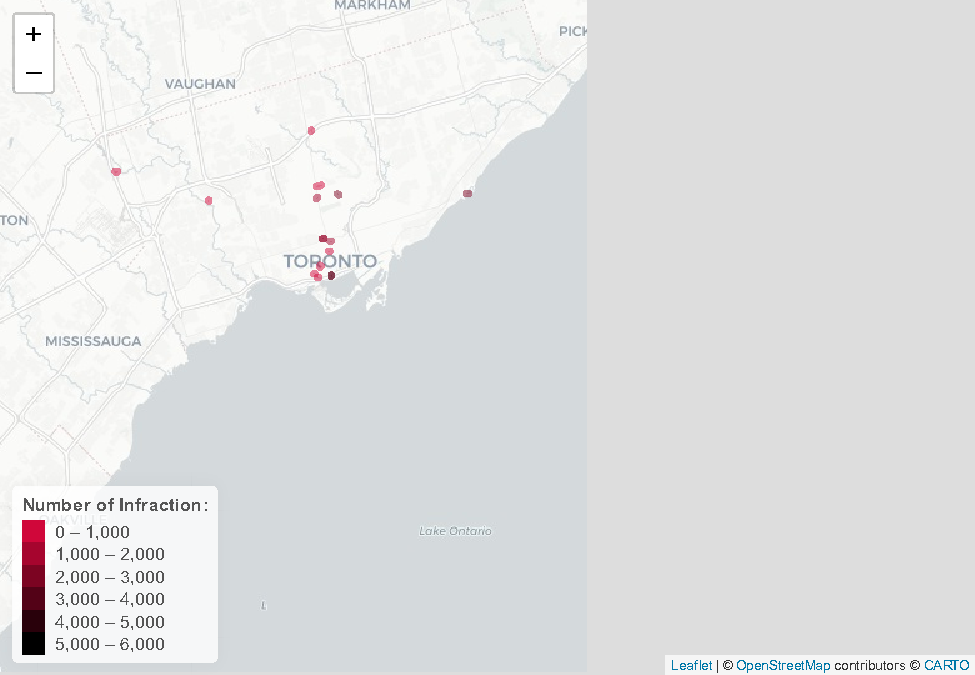
\includegraphics{main_1_files/figure-latex/Q1 plot-1.pdf}

\begin{Shaded}
\begin{Highlighting}[]
\NormalTok{GP\_metadata }\OtherTok{\textless{}{-}}\NormalTok{ opendatatoronto}\SpecialCharTok{::}\FunctionTok{show\_package}\NormalTok{(}\StringTok{"https://open.toronto.ca/dataset/green{-}p{-}parking/"}\NormalTok{)}
\NormalTok{GP\_list }\OtherTok{\textless{}{-}}\NormalTok{ opendatatoronto}\SpecialCharTok{::}\FunctionTok{list\_package\_resources}\NormalTok{(}\StringTok{"https://open.toronto.ca/dataset/green{-}p{-}parking/"}\NormalTok{)}
\NormalTok{GP\_retrieve }\OtherTok{\textless{}{-}} \ControlFlowTok{function}\NormalTok{(URL,No,format) \{}
\NormalTok{  list }\OtherTok{\textless{}{-}}\NormalTok{ opendatatoronto}\SpecialCharTok{::}\FunctionTok{list\_package\_resources}\NormalTok{(}\StringTok{"https://open.toronto.ca/dataset/green{-}p{-}parking/"}\NormalTok{)}
\NormalTok{  data\_id }\OtherTok{\textless{}{-}}\NormalTok{ list[[No, }\StringTok{"id"}\NormalTok{]]}
\NormalTok{  resource }\OtherTok{\textless{}{-}}
    \FunctionTok{resource\_show}\NormalTok{(data\_id, }\AttributeTok{url =} \StringTok{"https://ckan0.cf.opendata.inter.prod{-}toronto.ca/"}\NormalTok{, }\AttributeTok{as =} \StringTok{"list"}\NormalTok{)}
\NormalTok{  dir }\OtherTok{\textless{}{-}} \FunctionTok{tempdir}\NormalTok{()}
\NormalTok{  resource\_dir }\OtherTok{\textless{}{-}}\NormalTok{ fs}\SpecialCharTok{::}\FunctionTok{dir\_create}\NormalTok{(}\FunctionTok{paste0}\NormalTok{(dir, }\StringTok{"/"}\NormalTok{, data\_id))}
\NormalTok{  save\_path }\OtherTok{\textless{}{-}}
    \FunctionTok{ckan\_fetch}\NormalTok{(}
\NormalTok{      resource[[}\StringTok{"url"}\NormalTok{]],}
      \AttributeTok{store =} \StringTok{"disk"}\NormalTok{,}
      \AttributeTok{path =} \FunctionTok{paste0}\NormalTok{(dir, }\StringTok{"/"}\NormalTok{, data\_id, }\StringTok{"/"}\NormalTok{, }\StringTok{"res."}\NormalTok{,format)}
\NormalTok{    )}
\NormalTok{  GP\_json }\OtherTok{\textless{}{-}} \FunctionTok{fromJSON}\NormalTok{(}\AttributeTok{file =}\NormalTok{ save\_path[[}\StringTok{"path"}\NormalTok{]])}
\NormalTok{\}}

\NormalTok{GP\_json }\OtherTok{\textless{}{-}} \FunctionTok{GP\_retrieve}\NormalTok{(}\StringTok{"https://open.toronto.ca/dataset/green{-}p{-}parking/"}\NormalTok{,}\DecValTok{1}\NormalTok{,}\StringTok{"JSON"}\NormalTok{)}

\NormalTok{GP\_data }\OtherTok{\textless{}{-}} \FunctionTok{tibble}\NormalTok{(}\AttributeTok{id =} \DecValTok{1}\SpecialCharTok{:}\FunctionTok{length}\NormalTok{(GP\_json[[}\DecValTok{1}\NormalTok{]])) }\SpecialCharTok{\%\textgreater{}\%} 
  \FunctionTok{mutate}\NormalTok{(}\AttributeTok{address =} \FunctionTok{map\_chr}\NormalTok{(id,}\SpecialCharTok{\textasciitilde{}}\NormalTok{ GP\_json[[}\DecValTok{1}\NormalTok{]][[.x]]}\SpecialCharTok{$}\NormalTok{address),}
         \AttributeTok{lat =} \FunctionTok{as.double}\NormalTok{(}\FunctionTok{map\_chr}\NormalTok{(id,}\SpecialCharTok{\textasciitilde{}}\NormalTok{ GP\_json[[}\DecValTok{1}\NormalTok{]][[.x]]}\SpecialCharTok{$}\NormalTok{lat)),}
         \AttributeTok{lng =} \FunctionTok{as.double}\NormalTok{(}\FunctionTok{map\_chr}\NormalTok{(id,}\SpecialCharTok{\textasciitilde{}}\NormalTok{ GP\_json[[}\DecValTok{1}\NormalTok{]][[.x]]}\SpecialCharTok{$}\NormalTok{lng)),}
         \AttributeTok{rate =} \FunctionTok{map\_chr}\NormalTok{(id,}\SpecialCharTok{\textasciitilde{}}\NormalTok{ GP\_json[[}\DecValTok{1}\NormalTok{]][[.x]]}\SpecialCharTok{$}\NormalTok{rate)) }
\NormalTok{GP\_sf }\OtherTok{\textless{}{-}}\NormalTok{ GP\_data }\SpecialCharTok{\%\textgreater{}\%} 
  \FunctionTok{st\_as\_sf}\NormalTok{(}\AttributeTok{coords =} \FunctionTok{c}\NormalTok{(}\StringTok{"lng"}\NormalTok{, }\StringTok{"lat"}\NormalTok{),}
           \AttributeTok{crs =} \FunctionTok{st\_crs}\NormalTok{(}\DecValTok{4326}\NormalTok{))}
\end{Highlighting}
\end{Shaded}

\begin{Shaded}
\begin{Highlighting}[]
\NormalTok{PaTi\_GP }\OtherTok{\textless{}{-}} \FunctionTok{tibble}\NormalTok{()}
\NormalTok{PaTi\_GP\_over }\OtherTok{\textless{}{-}} \ControlFlowTok{function}\NormalTok{(r) \{}
\NormalTok{  GP\_sf\_buf }\OtherTok{\textless{}{-}}\NormalTok{ GP\_sf }\SpecialCharTok{\%\textgreater{}\%}
    \FunctionTok{st\_transform}\NormalTok{(}\DecValTok{3347}\NormalTok{) }\SpecialCharTok{\%\textgreater{}\%}
    \FunctionTok{st\_buffer}\NormalTok{(}\AttributeTok{dist =}\NormalTok{ r) }\SpecialCharTok{\%\textgreater{}\%}
    \FunctionTok{st\_transform}\NormalTok{(}\DecValTok{4326}\NormalTok{)}
  
  
\NormalTok{  GP\_sf\_buf }\SpecialCharTok{\%\textgreater{}\%} \FunctionTok{st\_intersects}\NormalTok{(PaTi\_polygon\_pl)}
\NormalTok{  sparse\_pl }\OtherTok{\textless{}{-}}
\NormalTok{    PaTi\_polygon\_pl }\SpecialCharTok{\%\textgreater{}\%} \FunctionTok{st\_intersects}\NormalTok{(GP\_sf\_buf, }\AttributeTok{sparse =}\NormalTok{ T)}
\NormalTok{  over\_pl }\OtherTok{\textless{}{-}}
    \FunctionTok{tibble}\NormalTok{(}\AttributeTok{infraction\_code =}\NormalTok{ PaTi\_polygon\_pl}\SpecialCharTok{$}\NormalTok{infraction\_code) }\SpecialCharTok{\%\textgreater{}\%}
    \FunctionTok{mutate}\NormalTok{(}
      \AttributeTok{row\_num =} \FunctionTok{row\_number}\NormalTok{(),}
      \AttributeTok{GP\_distance =}\NormalTok{ r,}
      \AttributeTok{no\_GP =} \FunctionTok{map\_dbl}\NormalTok{(row\_num,  }\SpecialCharTok{\textasciitilde{}} \FunctionTok{length}\NormalTok{(sparse\_pl[[.x]]))}
\NormalTok{    )}
  
\NormalTok{  GP\_sf\_buf }\SpecialCharTok{\%\textgreater{}\%} \FunctionTok{st\_intersects}\NormalTok{(PaTi\_polygon\_pt)}
\NormalTok{  sparse\_pt }\OtherTok{\textless{}{-}}
\NormalTok{    PaTi\_polygon\_pt }\SpecialCharTok{\%\textgreater{}\%} \FunctionTok{st\_intersects}\NormalTok{(GP\_sf\_buf, }\AttributeTok{sparse =}\NormalTok{ T)}
\NormalTok{  over\_pt }\OtherTok{\textless{}{-}}
    \FunctionTok{tibble}\NormalTok{(}\AttributeTok{infraction\_code =}\NormalTok{ PaTi\_polygon\_pt}\SpecialCharTok{$}\NormalTok{infraction\_code) }\SpecialCharTok{\%\textgreater{}\%}
    \FunctionTok{mutate}\NormalTok{(}
      \AttributeTok{row\_num =} \FunctionTok{row\_number}\NormalTok{(),}
      \AttributeTok{GP\_distance =}\NormalTok{ r,}
      \AttributeTok{no\_GP =} \FunctionTok{map\_dbl}\NormalTok{(row\_num,  }\SpecialCharTok{\textasciitilde{}} \FunctionTok{length}\NormalTok{(sparse\_pt[[.x]]))}
\NormalTok{    )}
  
\NormalTok{  res }\OtherTok{\textless{}{-}}\NormalTok{ over\_pl }\SpecialCharTok{\%\textgreater{}\%} \FunctionTok{rbind}\NormalTok{(over\_pt)}
\NormalTok{\}}

\ControlFlowTok{for}\NormalTok{ (r }\ControlFlowTok{in} \FunctionTok{seq}\NormalTok{(}\DecValTok{0}\NormalTok{,}\DecValTok{800}\NormalTok{,}\AttributeTok{by=}\DecValTok{50}\NormalTok{)) \{}
\NormalTok{  PaTi\_GP }\OtherTok{\textless{}{-}}\NormalTok{ PaTi\_GP }\SpecialCharTok{\%\textgreater{}\%} \FunctionTok{rbind}\NormalTok{(}\FunctionTok{PaTi\_GP\_over}\NormalTok{(r))}
\NormalTok{\}}


\NormalTok{PaTi\_GP\_tile }\OtherTok{\textless{}{-}}\NormalTok{ PaTi\_GP }\SpecialCharTok{\%\textgreater{}\%}
  \FunctionTok{ggplot}\NormalTok{()}\SpecialCharTok{+}
  \FunctionTok{geom\_raster}\NormalTok{(}\FunctionTok{aes}\NormalTok{(}\AttributeTok{x=}\FunctionTok{factor}\NormalTok{(infraction\_code,}\AttributeTok{levels =}\NormalTok{ PaTi\_data\_top20}\SpecialCharTok{$}\NormalTok{infraction\_code),}\AttributeTok{y=}\NormalTok{GP\_distance,}\AttributeTok{fill=}\NormalTok{no\_GP))}\SpecialCharTok{+} 
  \FunctionTok{theme\_bw}\NormalTok{()}\SpecialCharTok{+}
  \FunctionTok{theme}\NormalTok{(}\AttributeTok{axis.text.y =} \FunctionTok{element\_text}\NormalTok{(}\AttributeTok{vjust =} \FloatTok{1.5}\NormalTok{),}
        \AttributeTok{axis.ticks.y =} \FunctionTok{element\_blank}\NormalTok{()}\CommentTok{\#,}
        \CommentTok{\# panel.grid = element\_blank(),}
        \CommentTok{\# panel.border = element\_blank()}
\NormalTok{        )}\SpecialCharTok{+}
  \FunctionTok{scale\_x\_discrete}\NormalTok{(}\AttributeTok{name =} \StringTok{"Infraction code"}\NormalTok{,}\AttributeTok{expand=}\FunctionTok{c}\NormalTok{(}\DecValTok{0}\NormalTok{,}\DecValTok{0}\NormalTok{))}\SpecialCharTok{+}
  \FunctionTok{scale\_y\_continuous}\NormalTok{(}\AttributeTok{name =} \StringTok{"Green P Parking lot distance from}\SpecialCharTok{\textbackslash{}n}\StringTok{the most common location for an infraction code"}\NormalTok{,}\AttributeTok{expand=}\FunctionTok{c}\NormalTok{(}\DecValTok{0}\NormalTok{,}\DecValTok{0}\NormalTok{))}\SpecialCharTok{+}
  \FunctionTok{scale\_fill\_continuous}\NormalTok{(}\AttributeTok{name =} \StringTok{"number of}\SpecialCharTok{\textbackslash{}n}\StringTok{Green P}\SpecialCharTok{\textbackslash{}n}\StringTok{parking lots"}\NormalTok{)}
  
\FunctionTok{plot}\NormalTok{(PaTi\_GP\_tile)}
\end{Highlighting}
\end{Shaded}

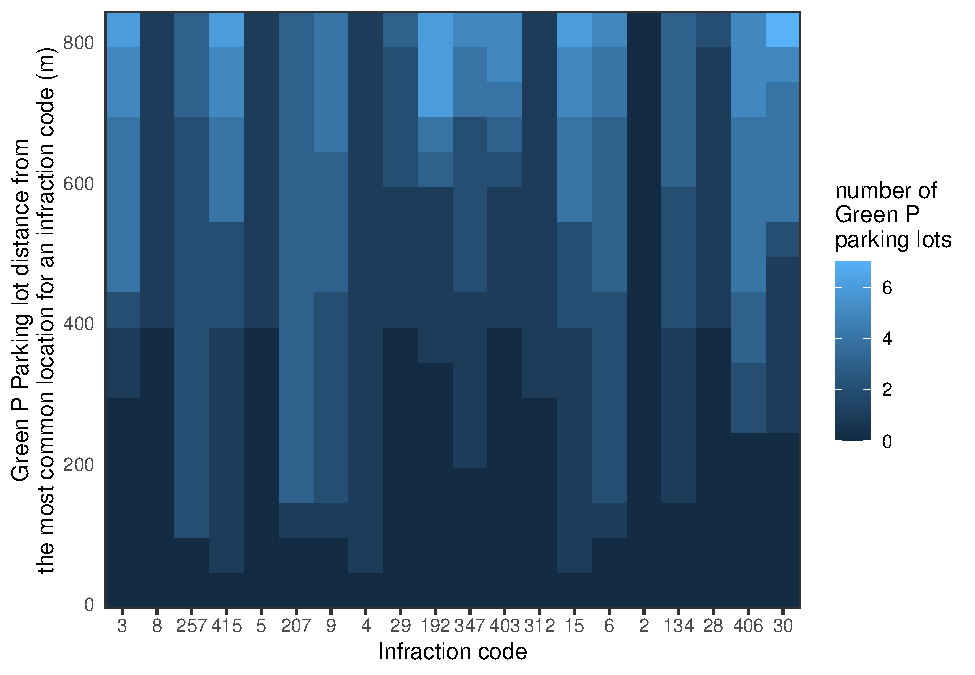
\includegraphics{main_1_files/figure-latex/Green P tile-1.pdf}

\begin{Shaded}
\begin{Highlighting}[]
\NormalTok{PaTi\_GP\_over\_id }\OtherTok{\textless{}{-}} \ControlFlowTok{function}\NormalTok{(r) \{}
\NormalTok{  GP\_sf\_buf }\OtherTok{\textless{}{-}}\NormalTok{ GP\_sf }\SpecialCharTok{\%\textgreater{}\%}
    \FunctionTok{st\_transform}\NormalTok{(}\DecValTok{3347}\NormalTok{) }\SpecialCharTok{\%\textgreater{}\%}
    \FunctionTok{st\_buffer}\NormalTok{(}\AttributeTok{dist =}\NormalTok{ r) }\SpecialCharTok{\%\textgreater{}\%}
    \FunctionTok{st\_transform}\NormalTok{(}\DecValTok{4326}\NormalTok{)}
  
  
\NormalTok{  GP\_sf\_buf }\SpecialCharTok{\%\textgreater{}\%} \FunctionTok{st\_intersects}\NormalTok{(PaTi\_polygon\_pl)}
\NormalTok{  sparse\_pl }\OtherTok{\textless{}{-}}
\NormalTok{    PaTi\_polygon\_pl }\SpecialCharTok{\%\textgreater{}\%} \FunctionTok{st\_intersects}\NormalTok{(GP\_sf\_buf, }\AttributeTok{sparse =}\NormalTok{ T)}
  
  
\NormalTok{  GP\_sf\_buf }\SpecialCharTok{\%\textgreater{}\%} \FunctionTok{st\_intersects}\NormalTok{(PaTi\_polygon\_pt)}
\NormalTok{  sparse\_pt }\OtherTok{\textless{}{-}}
\NormalTok{    PaTi\_polygon\_pt }\SpecialCharTok{\%\textgreater{}\%} \FunctionTok{st\_intersects}\NormalTok{(GP\_sf\_buf, }\AttributeTok{sparse =}\NormalTok{ T)}
  
\NormalTok{  res }\OtherTok{\textless{}{-}} \FunctionTok{unique}\NormalTok{(}\FunctionTok{c}\NormalTok{(}\FunctionTok{unlist}\NormalTok{(sparse\_pl),}\FunctionTok{unlist}\NormalTok{(sparse\_pt)))}
  
  \FunctionTok{return}\NormalTok{(res)}
\NormalTok{\}}

\NormalTok{PaTi\_GP\_400\_id }\OtherTok{\textless{}{-}} \FunctionTok{PaTi\_GP\_over\_id}\NormalTok{(}\DecValTok{400}\NormalTok{)}
\NormalTok{GP\_sf\_buf }\OtherTok{\textless{}{-}}\NormalTok{ GP\_sf[PaTi\_GP\_400\_id,] }\SpecialCharTok{\%\textgreater{}\%}
    \FunctionTok{st\_transform}\NormalTok{(}\DecValTok{3347}\NormalTok{) }\SpecialCharTok{\%\textgreater{}\%}
    \FunctionTok{st\_buffer}\NormalTok{(}\AttributeTok{dist =} \DecValTok{400}\NormalTok{) }\SpecialCharTok{\%\textgreater{}\%}
    \FunctionTok{st\_transform}\NormalTok{(}\DecValTok{4326}\NormalTok{)}

\NormalTok{PaTi\_GP\_400\_plot }\OtherTok{\textless{}{-}} \FunctionTok{leaflet}\NormalTok{() }\SpecialCharTok{\%\textgreater{}\%} 
  \FunctionTok{addProviderTiles}\NormalTok{(providers}\SpecialCharTok{$}\NormalTok{CartoDB.Positron) }\SpecialCharTok{\%\textgreater{}\%} 
  \FunctionTok{addPolygons}\NormalTok{(}\AttributeTok{data =}\NormalTok{ PaTi\_polygon\_pl,}
              \AttributeTok{popup=}\FunctionTok{paste}\NormalTok{(}\CommentTok{\#"\textless{}b\textgreater{}Infraction Code\textless{}/b\textgreater{}",PaTi\_polygon\_pl$infraction\_code,"\textless{}br\textgreater{}",}
                          \StringTok{"\textless{}b\textgreater{}Description:\textless{}/b\textgreater{}"}\NormalTok{,PaTi\_polygon\_pl}\SpecialCharTok{$}\NormalTok{infraction\_description,}\StringTok{"\textless{}br\textgreater{}"}\NormalTok{,}
                          \StringTok{"\textless{}b\textgreater{}Location:\textless{}/b\textgreater{}"}\NormalTok{,PaTi\_polygon\_pl}\SpecialCharTok{$}\NormalTok{LFNAME,}\StringTok{"\textless{}br\textgreater{}"}\NormalTok{,}
                          \StringTok{"\textless{}b\textgreater{}Number of Infraction:\textless{}/b\textgreater{}"}\NormalTok{,PaTi\_polygon\_pl}\SpecialCharTok{$}\NormalTok{no\_infraction,}\StringTok{"\textless{}br\textgreater{}"}\NormalTok{,}
                          \StringTok{"\textless{}b\textgreater{}Infraction Fine:\textless{}/b\textgreater{}"}\NormalTok{,}\FunctionTok{dollar\_format}\NormalTok{()(PaTi\_polygon\_pl}\SpecialCharTok{$}\NormalTok{set\_fine\_amount),}\StringTok{"\textless{}br\textgreater{}"}\NormalTok{),}
              \AttributeTok{label =} \SpecialCharTok{\textasciitilde{}} \FunctionTok{paste0}\NormalTok{(}\StringTok{"Infraction Code "}\NormalTok{, infraction\_code),}
              \AttributeTok{color =} \StringTok{"\#6e031e"}\NormalTok{) }\SpecialCharTok{\%\textgreater{}\%} 
  \FunctionTok{addPolygons}\NormalTok{(}\AttributeTok{data =}\NormalTok{ PaTi\_polygon\_pt,}
              \AttributeTok{popup=}\FunctionTok{paste}\NormalTok{(}
                          \StringTok{"\textless{}b\textgreater{}Description:\textless{}/b\textgreater{}"}\NormalTok{,PaTi\_polygon\_pt}\SpecialCharTok{$}\NormalTok{infraction\_description,}\StringTok{"\textless{}br\textgreater{}"}\NormalTok{,}
                          \StringTok{"\textless{}b\textgreater{}Location:\textless{}/b\textgreater{}"}\NormalTok{,PaTi\_polygon\_pt}\SpecialCharTok{$}\NormalTok{LFNAME,}\StringTok{"\textless{}br\textgreater{}"}\NormalTok{,}
                          \StringTok{"\textless{}b\textgreater{}Number of Infraction:\textless{}/b\textgreater{}"}\NormalTok{,PaTi\_polygon\_pt}\SpecialCharTok{$}\NormalTok{no\_infraction,}\StringTok{"\textless{}br\textgreater{}"}\NormalTok{,}
                          \StringTok{"\textless{}b\textgreater{}Infraction Fine:\textless{}/b\textgreater{}"}\NormalTok{,}\FunctionTok{dollar\_format}\NormalTok{()(PaTi\_polygon\_pt}\SpecialCharTok{$}\NormalTok{set\_fine\_amount),}\StringTok{"\textless{}br\textgreater{}"}\NormalTok{),}
              \AttributeTok{label =} \SpecialCharTok{\textasciitilde{}} \FunctionTok{paste0}\NormalTok{(}\StringTok{"Infraction Code "}\NormalTok{, infraction\_code),}
              \AttributeTok{color =} \StringTok{"\#6e031e"}\NormalTok{) }\SpecialCharTok{\%\textgreater{}\%} 
  \FunctionTok{addPolygons}\NormalTok{(}\AttributeTok{data =}\NormalTok{ GP\_sf\_buf,}
              \AttributeTok{popup=}\FunctionTok{paste}\NormalTok{(}
                          \StringTok{"\textless{}b\textgreater{}Address:\textless{}/b\textgreater{}"}\NormalTok{,GP\_sf\_buf}\SpecialCharTok{$}\NormalTok{address,}\StringTok{"\textless{}br\textgreater{}"}\NormalTok{,}
                          \StringTok{"\textless{}b\textgreater{}Rate:\textless{}/b\textgreater{}"}\NormalTok{,GP\_sf\_buf}\SpecialCharTok{$}\NormalTok{rate),}
              \AttributeTok{label =} \SpecialCharTok{\textasciitilde{}} \FunctionTok{paste0}\NormalTok{(}\StringTok{"Green P id: "}\NormalTok{, id),}
              \AttributeTok{color =} \StringTok{"green"}\NormalTok{) }\CommentTok{\#\%\textgreater{}\% }

\NormalTok{PaTi\_GP\_400\_plot}
\end{Highlighting}
\end{Shaded}

\includegraphics{main_1_files/figure-latex/Green P map-1.pdf}

Add a new chunk by clicking the \emph{Insert Chunk} button on the
toolbar or by pressing \emph{Ctrl+Alt+I}.

When you save the notebook, an HTML file containing the code and output
will be saved alongside it (click the \emph{Preview} button or press
\emph{Ctrl+Shift+K} to preview the HTML file).

The preview shows you a rendered HTML copy of the contents of the
editor. Consequently, unlike \emph{Knit}, \emph{Preview} does not run
any R code chunks. Instead, the output of the chunk when it was last run
in the editor is displayed.

\end{document}
